% This template mostly comes from Yiyang JIANG


\documentclass{beamer}
\usepackage{ctex, hyperref}
\usepackage[T1]{fontenc}

% other packages
\usepackage{latexsym,amsmath,xcolor,multicol,booktabs,calligra}
\usepackage{graphicx,pstricks,listings,stackengine}

\author{\href{}{Your Name(XXXXXXXXXd)}}
\institute{\href{}{Deparment of Computing, The Hong Kong Polytechnic University}}
\title{Presentation Name}
\subtitle{}
\date{}
\usepackage{JYY_Beamer}

% defs
\def\cmd#1{\texttt{\color{red}\footnotesize $\backslash$#1}}
\def\env#1{\texttt{\color{blue}\footnotesize #1}}
\definecolor{deepblue}{rgb}{0,0,0.5}
\definecolor{deepred}{rgb}{0.6,0,0}
\definecolor{deepgreen}{rgb}{0,0.5,0}
\definecolor{halfgray}{gray}{0.55}

\lstset{
    basicstyle=\ttfamily\small,
    keywordstyle=\bfseries\color{deepblue},
    emphstyle=\ttfamily\color{deepred},   % Custom highlighting style
    stringstyle=\color{deepgreen},
    numbers=left,
    numberstyle=\small\color{halfgray},
    rulesepcolor=\color{red!20!green!20!blue!20},
    frame=shadowbox,
}


\begin{document}

\kaishu
\begin{frame}
    \titlepage
    \begin{figure}[htpb]
        \begin{center}
            
\includegraphics[width=0.45\linewidth]{pic/polyu.png}
        \end{center}
    \end{figure}
\end{frame}

\begin{frame}
    \tableofcontents[sectionstyle=show,subsectionstyle=show/shaded/hide,subsubsectionstyle=show/shaded/hide]
\end{frame}


% 内容从这里开始
\section{Background}

\begin{frame}{Introduction}
%    \begin{block}{haha}
% asdfsdf
% \end{block} 

\begin{itemize}
    \item One
    \item Two
    
\end{itemize}

\end{frame}


\section{First Item}
\begin{frame}{Second}

\begin{itemize}
    \item Training set: XXX columns, YYY samples, 79x more training than test data.
    \item Test set: XXX samples, YYY irregular features, binary targets. 
    \begin{itemize}
        \item 50\% value is 1, 50\% value is 0.
    \end{itemize}
\end{itemize}
    
\end{frame}

\begin{frame}{Third}
\begin{itemize}
    \item Feature data variance: X.XX to X.XX (range of $1\pm0.XX$).
    \item Feature data mean: 0.XX to -0.XX (range of $0\pm0.XX$).
\end{itemize}
\end{frame}

\begin{frame}{Figure Frame}
    \begin{figure}
        \centering
        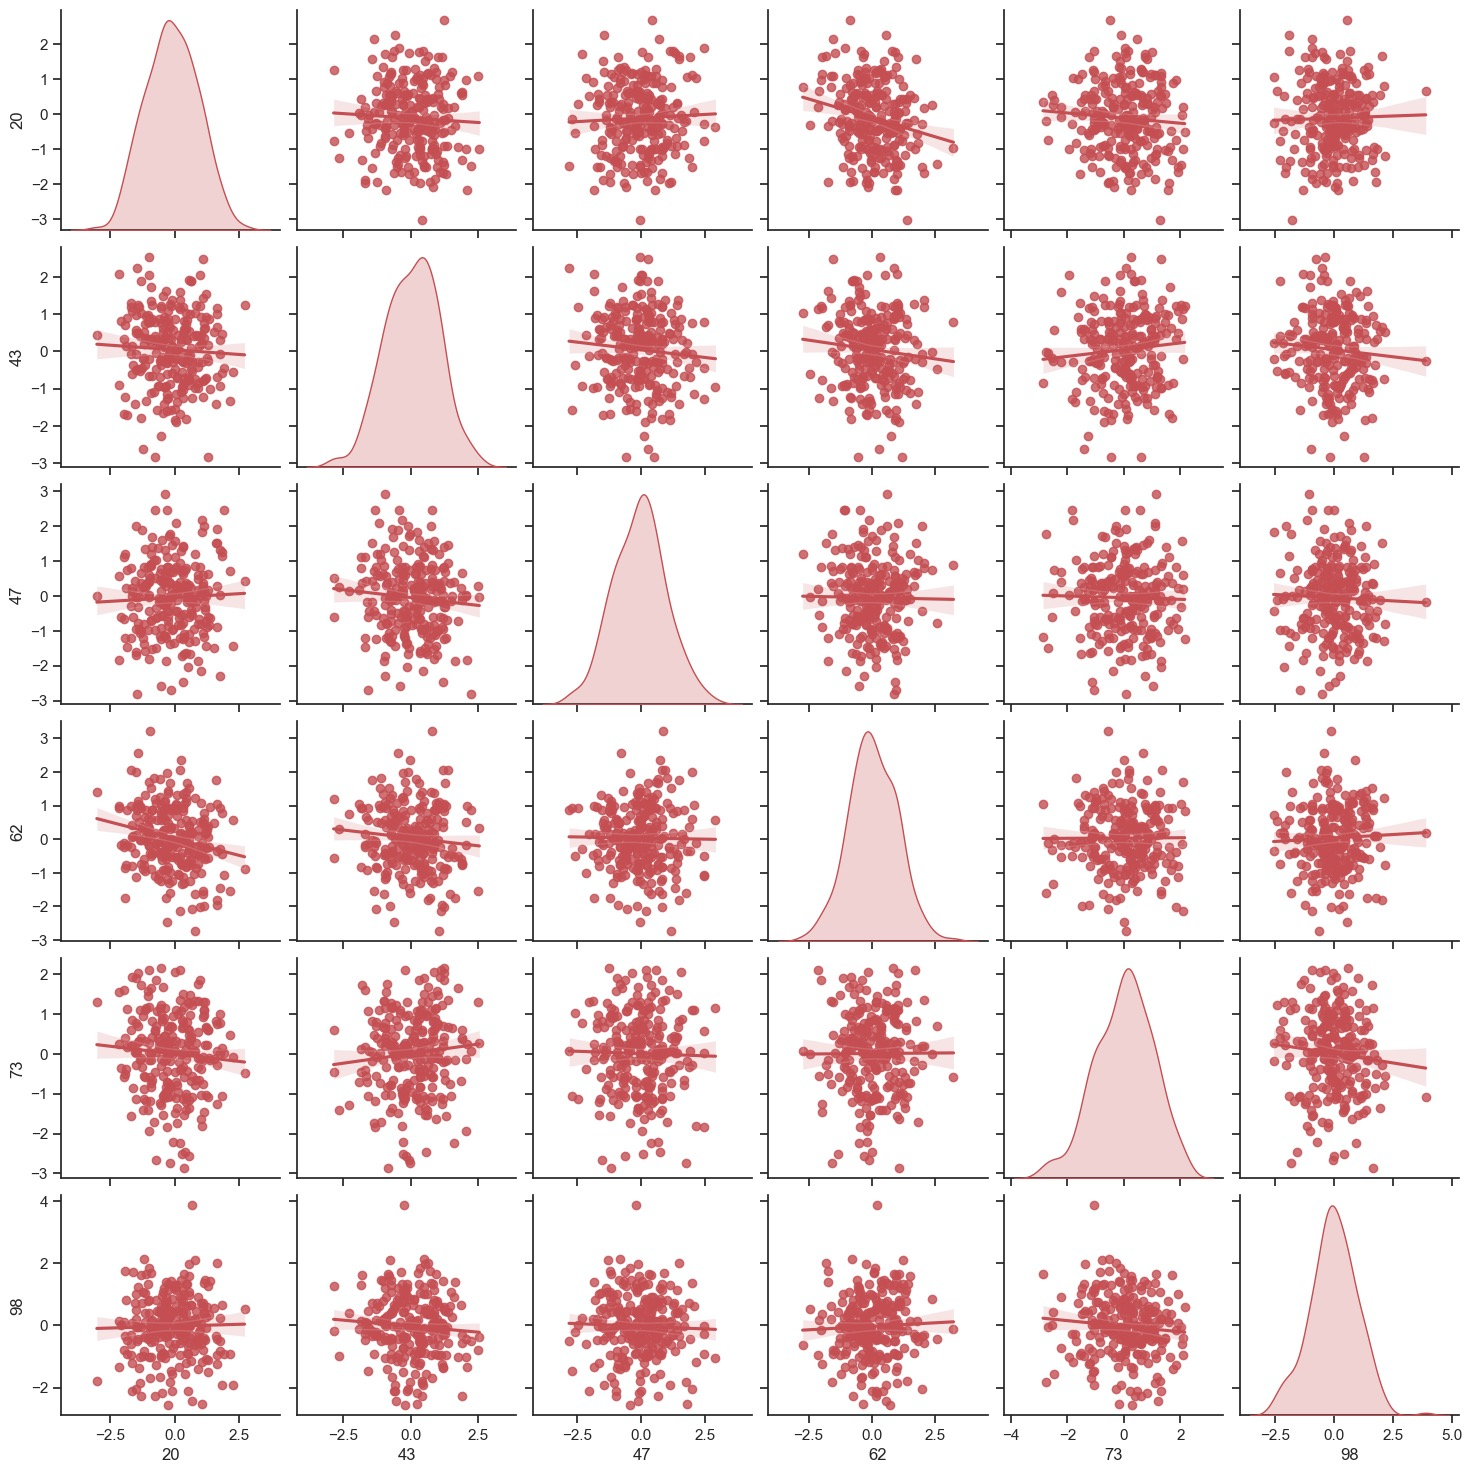
\includegraphics[width = 7cm, height = 6cm]{pic/fig1.jpg}
        \caption{Your figure name}
        \label{fig:my_label}
    \end{figure}
\end{frame}



\begin{frame}{Table Frame}

\begin{table}
\begin{tabular}{c|cc}
C ($\frac{1}{\lambda}$) & Cross validation Score & Submission Score \\
\hline
1            & 1                      & 0.82             \\
0.5          & 1                      & 0.83             \\
0.2          & 1                      & 0.845            \\
0.1          & 0.9048                 & 0.849            \\
0.15         & 0.9643                 & 0.846            \\
0.05         & 0.7619                 & 0.787           
\end{tabular}
\caption{Your table name}
\label{table:1}
\end{table}

\end{frame}


\section{Conclusion}
\begin{frame}{Conclusion}
\begin{itemize}
\item Your conclusion

\end{itemize}
\end{frame}


\section{References}

\begin{frame}{References}

\nocite{bibitem1}
\nocite{*}
\bibliographystyle{IEEEtran} 
\bibliography{ref}


\end{frame}



\end{document}
